\subsection{Trục số một chiều}

\ % Lùi đầu dòng

Đồ thị là cầu nối đầu tiên giữa đại số và hình học mà chắc là bạn đọc đã được học. Thông thường, nhắc đến đồ thị, chúng thường được dùng để biểu thị mặt phẳng hai chiều hoặc không gian ba chiều. Nhưng, đồ thị cơ bản nhất chỉ có một chiều, hay tên gọi khác là \emph{trục số}. 

\def \pointSize {1.5pt}

\begin{wrapfigure}{R}{0.4\textwidth}
   \centering
   \begin{tikzpicture}
      \draw[->] (-3,0) -- (2,0) node[right] {Trục số};
      \filldraw (0, 0) circle (\pointSize) node[below] {$O(0)$};
      \filldraw (1.5, 0) circle (\pointSize) node[below] {$P(x_P)$};
      \filldraw (-1.5, 0) circle (\pointSize) node[below] {$P_-(-x_P)$};
   \end{tikzpicture}
   \caption{Trục số một chiều}
   \label{fig:do_thi:truc_so:truc_so_mot_chieu}
\end{wrapfigure}

Đặt một điểm trên trục làm gốc tọa độ $0$, từ đó chúng ta có thể biểu diễn mọi số thực trên trục số này. Nói một cách không chính thống, với một số $x_P$ dương bất kì, đánh dấu cách $O$ một đoạn bằng $x_P$ đơn vị độ dài theo hướng trục, chúng ta có điểm $P$ biểu diễn $x_P$. Viết tắt cách biểu diễn, được $P(x_P)$. Ngược lại, nếu chúng ta muốn đánh dấu số $x_{P_-}=-x_P$ mang giá trị âm, chúng ta dịch ngược lại chiều trục như trên hình \ref{fig:do_thi:truc_so:truc_so_mot_chieu}.

\begin{wrapfigure}{R}{0.4\textwidth}
   \centering
   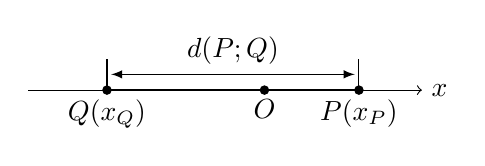
\begin{tikzpicture}
      \draw[->] (-3,0) -- (2,0) node[right] {$x$};
      \filldraw (0, 0) circle (\pointSize) node[below] {$O$};
      \pgfmathsetmacro{\xP}{1.2}
      \pgfmathsetmacro{\xQ}{-2}
      \pgfmathsetmacro{\h}{0.4}
      \filldraw (\xP, 0) circle (\pointSize) node[below] {$P(x_P)$};
      \filldraw (\xQ, 0) circle (\pointSize) node[below] {$Q(x_Q)$};
      \draw[thick] (\xQ,0) -- (\xP,0);
      \node[above] at ({(\xP+\xQ)/2}, {\h/2}) {$d(P;Q)$};
      \draw (\xP,0) -- (\xP,\h);
      \draw (\xQ,0) -- (\xQ,\h);
      \draw[<->, >=latex, shorten >=\pointSize, shorten <=\pointSize] (\xP,{\h/2}) -- (\xQ,{\h/2});
   \end{tikzpicture}
   \caption{Khoảng cách trên trục số}
   \label{fig:do_thi:truc_so:khoang_cach_truc_so}
\end{wrapfigure}

Khi có nhiều điểm ở trên đồ thị, chúng ta sẽ mong muốn tính những thông số liên quan tới những điểm đó. Do kiến thức toán hiện tại đang bị giới hạn, chúng ta sẽ chỉ tập trung vào một đặc điểm nhất định, \emph{khoảng cách}. Trên một trục số như hình \ref{fig:do_thi:truc_so:khoang_cach_truc_so}, cho hai điểm $P(x_P)$ và $Q(x_Q)$, khoảng cách giữa chúng là $$d(P;Q)=\sqrt{(x_P-x_Q)^2}=|x_P-x_Q|.$$

\exercise[ex:0.1] Biểu diễn nhóm các điểm sau trên trục số. Tính khoảng cách giữa hai điểm phân biệt bất kì trong nhóm đó.
\begin{enumerate}
   \item $A(2)$, $B(-3)$, và $C(4)$;
   \item $D(\pi)$, $E(-\pi)$, $F(0)$, và $G\left(\frac{\pi}{2}\right)$;
   \item $H(0{,}\overline{3})$ và $I(\sqrt{2})$;
   \item $J\left(\frac{355}{113}\right)$, $K\left(\frac{9801}{2206\sqrt{2}}\right)$ và $L\left(\sqrt[4]{\frac{2143}{22}}\right)$;
   \item $M(x)$ và $N(2x)$ với $x\in\mathbb{R}$.
\end{enumerate}

\solution[ex:0.1] 
\begin{figure}[h]
   \centering
   \fbox{  
      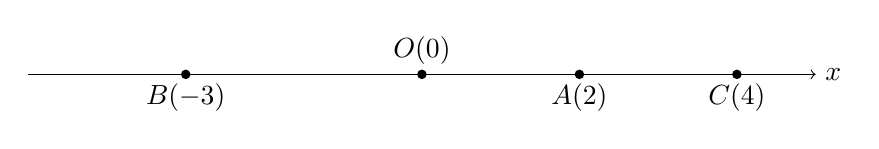
\begin{tikzpicture}
         \draw[->] (-5,0) -- (5,0) node[right] {$x$};
         \filldraw (0, 0) circle (\pointSize) node[above] {$O(0)$};
         \filldraw (2, 0) circle (\pointSize) node[below] {$A(2)$};
         \filldraw (-3, 0) circle (\pointSize) node[below] {$B(-3)$};
         \filldraw (4, 0) circle (\pointSize) node[below] {$C(4)$};
      \end{tikzpicture}
   }
   \caption{Trục số cho phần 1 của bài \ref{ex:0.1}}
   \label{fig:do_thi:truc_so:truc_so_nguyen}
\end{figure}

\begin{figure}[h]
   \centering
   \fbox{  
      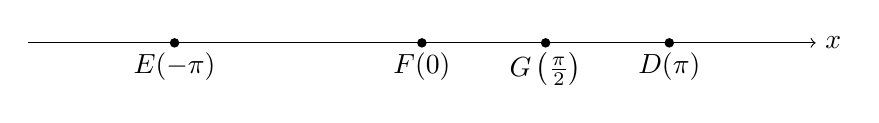
\begin{tikzpicture}
         \draw[->] (-5,0) -- (5,0) node[right] {$x$};
         \filldraw ({pi}, 0) circle (\pointSize) node[below] {$D(\pi)$};
         \filldraw ({-pi}, 0) circle (\pointSize) node[below] {$E(-\pi)$};
         \filldraw (0, 0) circle (\pointSize) node[below] {$F(0)$};
         \filldraw ({pi/2}, 0) circle (\pointSize) node[below] {$G\left(\frac{\pi}{2}\right)$};
      \end{tikzpicture}
   }
   \caption{Trục số cho phần 2 của bài \ref{ex:0.1}}
   \label{fig:do_thi:truc_so:truc_so_pi}
\end{figure}

\begin{figure}[h]
   \centering
   \fbox{
      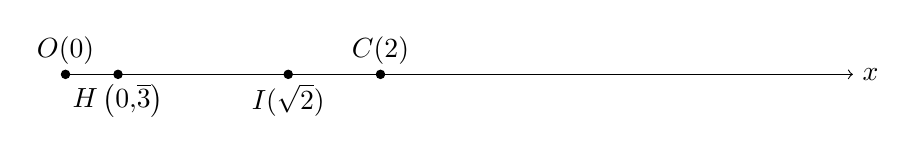
\begin{tikzpicture}
         \draw[->] (0,0) -- (10,0) node[right] {$x$};
         \filldraw (0, 0) circle (\pointSize) node[above] {$O(0)$};
         \filldraw ({2/3}, 0) circle (\pointSize) node[below] {$H\left(0{,}\overline{3}\right)$};
         \filldraw ({2*sqrt(2)}, 0) circle (\pointSize) node[below] {$I(\sqrt{2})$};
         \filldraw (4, 0) circle (\pointSize) node[above] {$C(2)$};
      \end{tikzpicture}
   }
   \caption{Trục số cho phần 3 của bài \ref{ex:0.1}}
   \label{fig:do_thi:truc_so:truc_so_thap_phan}
\end{figure}

\begin{figure}[h]
   \centering
   \fbox{
      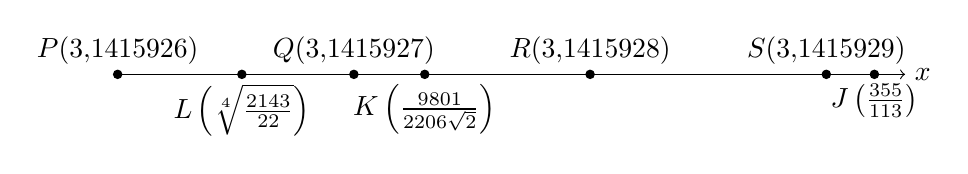
\begin{tikzpicture}
         \draw[->] (0,0) -- (10,0) node[right] {$x$};
         \filldraw (0,0) circle (\pointSize) node[above] {$P(3{,}1415926)$};
         \filldraw (3,0) circle (\pointSize) node[above] {$Q(3{,}1415927)$};
         \filldraw (6,0) circle (\pointSize) node[above] {$R(3{,}1415928)$};
         \filldraw (9,0) circle (\pointSize) node[above] {$S(3{,}1415929)$};
         \filldraw (9.61062, 0) circle (\pointSize) node[below] {$J\left(\frac{355}{113}\right)$};
         \filldraw (3.9, 0) circle (\pointSize) node[below] {$K\left(\frac{9801}{2206\sqrt{2}}\right)$};
         \filldraw (1.577475, 0) circle (\pointSize) node[below] {$L\left(\sqrt[4]{\frac{2143}{22}}\right)$};
      \end{tikzpicture}
   }
   \caption{Trục số cho phần 4 của bài \ref{ex:0.1}}
   \label{fig:do_thi:truc_so:truc_so_xap_xi_pi}
\end{figure}



Ta có đồ thị cho các phần từ $1$ đến $4$ như các hình \ref{fig:do_thi:truc_so:truc_so_nguyen}, \ref{fig:do_thi:truc_so:truc_so_pi}, \ref{fig:do_thi:truc_so:truc_so_thap_phan}, và \ref{fig:do_thi:truc_so:truc_so_xap_xi_pi}.

Cần lưu ý rằng, để biểu diễn thuận lợi nhất, các trục số khi biểu diễn số cần được chọn những tỉ lệ khác nhau và tại những vị trí khác nhau.

Các khoảng cách giữa hai điểm phân biệt đôi một là
\begin{enumerate}
   \item \begin{alignat*}{2}
      &d(A;B) = d(B;A) = \left|2 - (-3)\right| = \boxed{5}; \\
      &d(B;C) = d(C;B) = \left|4 - (-3)\right| = \boxed{7}; \\
      &d(C;A) = d(A;C) = \left|4 - 2\right| = \boxed{2}.
   \end{alignat*}
   \item \begin{alignat*}{2}
      &d(D;E) = d(E;D) = \left|\pi - (-\pi)\right| = \boxed{2\pi}; \\
      &d(E;F) = d(F;E) = \left|(-\pi) - 0\right| = \boxed{\pi}; \\
      &d(F;G) = d(G;F) = \left|0 - \frac{\pi}{2}\right| = \boxed{\frac{\pi}{2}}; \\
      &d(G;D) = d(D;G) = \left|\frac{\pi}{2} - \pi\right| = \boxed{\frac{\pi}{2}}; \\
      &d(D;F) = d(F;D) = \left|\pi - 0\right| = \boxed{\pi};\\
      &d(E;G) = d(G;E) = \left|(-\pi) - \frac{\pi}{2}\right| = \boxed{\frac{3\pi}{2}}.
   \end{alignat*}
   \item \begin{alignat*}{2}
      &d(H;I) = d(I;H) = \left|0{,}\overline{3} - \sqrt{2}\right| = \boxed{\frac{1-3\sqrt{2}}{3}}.
   \end{alignat*}
   \item \begin{alignat*}{2}
      &d(J;K) = d(K;J) = \left|\frac{355}{113} - \frac{9801}{2206\sqrt{2}}\right| = \boxed{\frac{1566260-1107513\sqrt{2}}{498556} \approx 1{,}9034\times 10^{-7}}; \\
      &d(K;L) = d(L;K) = \left|\frac{9801}{2206\sqrt{2}} - \sqrt[4]{\frac{2143}{22}}\right| = \boxed{\frac{107811\sqrt{2}-2206\sqrt[4]{22818664}}{48532} \approx 7{,}7431\times 10^{-8}}; \\
      &d(L;J) = d(J;L) = \left|\sqrt[4]{\frac{2143}{22}} - \frac{355}{113}\right| = \boxed{\frac{7810-113\sqrt[4]{22818664}}{2486} \approx 2{,}6777\times 10^{-7}}.
   \end{alignat*}
\end{enumerate}

\begin{figure}[h]
   \centering
   \fbox{
      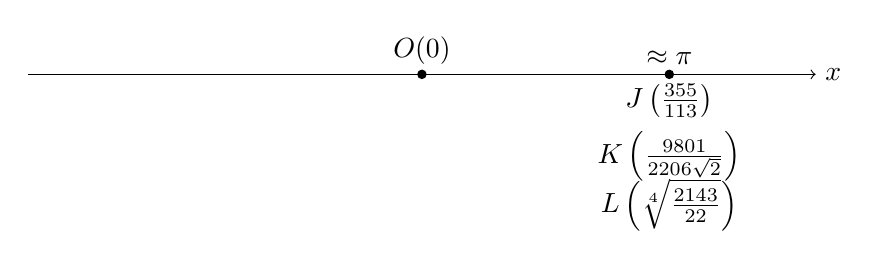
\begin{tikzpicture}
         \draw[->] (-5,0) -- (5,0) node[right] {$x$};
         \filldraw (0, 0) circle (\pointSize) node[above] {$O(0)$};
         \filldraw (pi, 0) circle (\pointSize) node[below] {$J\left(\frac{355}{113}\right)$};
         \node[below] at (pi, -0.6) {$K\left(\frac{9801}{2206\sqrt{2}}\right)$};
         \node[below] at (pi, -1.2) {$L\left(\sqrt[4]{\frac{2143}{22}}\right)$};
         \node[above] at (pi, 0) {$\approx \pi$};
      \end{tikzpicture}
   }
   \caption{Xấp xỉ vị trí điểm trên trục số cho phần $4$ của bài \ref{ex:0.1}}
   \label{fig:do_thi:truc_so:truc_so_bon_xx}
\end{figure}

Trong vật lí, việc tính toán chính xác đến như ở phần $4$ là không cần thiết và nhiều khi còn không chính xác. Luôn luôn có sai số khi đo đạc, và trong phần lớn trường hợp, khi kết hợp sai số này vào trong tính toán thì các giá trị khoảng cách như trên gần như vô nghĩa. Cho nên, về mặt thực tiễn, chúng ta hoàn toàn có thể thay thế đồ thị của $4$ như hình \ref{fig:do_thi:truc_so:truc_so_bon_xx} và khi tính khoảng cách, chúng ta có thể tính xấp xỉ là $$d(J,K) = d(K,J) \approx d(K,L) = d(L,K) \approx d(L,J) = d(J,L) \boxed{\approx 0}.$$

\begin{figure}[h]
   \centering
   \fbox{
      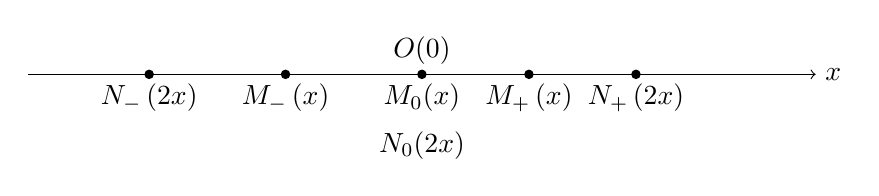
\begin{tikzpicture}
         \draw[->] (-5,0) -- (5,0) node[right] {$x$};
         \filldraw (0, 0) circle (\pointSize) node[above] {$O(0)$} node[below] {$M_0(x)$};
         \node[below] at (0, -0.6) {$N_0(2x)$};
         \filldraw ({e / 2}, 0) circle (\pointSize) node[below] {$M_+\left(x\right)$};
         \filldraw (e, 0) circle (\pointSize) node[below] {$N_+\left(2x\right)$};
         \filldraw ({-sqrt(3)}, 0) circle (\pointSize) node[below] {$M_-\left(x\right)$};
         \filldraw ({-sqrt(3) * 2}, 0) circle (\pointSize) node[below] {$N_-\left(2x\right)$};
      \end{tikzpicture}
   }
   \caption{Ba trường hợp cho vị trí tương đối của $M$, $N$, $O$ cho phần $5$ của bài \ref{ex:0.1}}
   \label{fig:truc phan 5}
\end{figure}

Để vẽ được đồ thị cho phần $5$, chúng ta sẽ xét vị trí tương đối giữa $M$, $N$ kèm theo gốc $O$ để quy chiếu như biểu diễn ở hình \ref{fig:truc phan 5}. Cụ thể, khi $x>0$, điểm $M$ và $N$ được biểu diễn thành hai điểm $M_+$ và $N_+$. Tương tự, khi $x<0$, $M$ và $N$ biểu diễn hai điểm $M_-$ và $N_-$. Một trường hợp đặc biệt là khi $x=0$, $M$ và $N$ đều có tọa độ là $0$, cho nên hai điểm đó và gốc cùng chia sẻ vị trí với nhau.

Khoảng cách giữa hai điểm $M$ và $N$ luôn là $$d(M;N)=d(N;M)=|x-2x|=\boxed{|x|}.$$